\documentclass{beamer} % [mathserif]
\usepackage{amsmath}
\usepackage{graphicx}
\usepackage{subfigure}
\usepackage{wrapfig}
\usepackage{booktabs}
\usepackage{hyperref}
\usepackage{pgfplots}
\pgfplotsset{compat=1.18}
\usepgfplotslibrary{dateplot}
\usepackage{tipa}
% \usepackage{epstopdf} % this is needed for windows Texworks
\usepackage[absolute,overlay]{textpos} % ,showboxes

\setlength{\TPHorizModule}{1in}
\TPVertModule=\TPHorizModule

\DeclareGraphicsExtensions{.eps}

\usetheme{Marburg}
% \usetheme{Berkeley}
% \usecolortheme{rose}
\definecolor{naublue}{HTML}{002454}
\definecolor{nauyellow}{HTML}{FAC01A}
%\setbeamercolor{structure}{bg=nauyellow, fg=naublue}
\setbeamercolor{palette primary}{bg=nauyellow, fg=naublue}
\setbeamercolor{palette secondary}{bg=nauyellow, fg=naublue}
%%%% See https://en.wikibooks.org/wiki/LaTeX/Presentations#User-defined_themes
% \setbeamercolor{alerted text}{fg=orange}
% \setbeamercolor{background canvas}{bg=white}
% \setbeamercolor{block body alerted}{bg=normal text.bg!90!black}
% \setbeamercolor{block body}{bg=normal text.bg!90!black}
% \setbeamercolor{block body example}{bg=normal text.bg!90!black}
% \setbeamercolor{block title alerted}{use={normal text,alerted text},fg=alerted text.fg!75!normal text.fg,bg=normal text.bg!75!black}
% \setbeamercolor{block title}{bg=blue}
% \setbeamercolor{block title example}{use={normal text,example text},fg=example text.fg!75!normal text.fg,bg=normal text.bg!75!black}
% \setbeamercolor{fine separation line}{}
\setbeamercolor{frametitle}{fg=naublue}
% \setbeamercolor{item projected}{fg=black}
% \setbeamercolor{normal text}{bg=black,fg=yellow}
% \setbeamercolor{palette sidebar primary}{use=normal text,fg=normal text.fg}
\setbeamercolor{palette sidebar primary}{bg=naublue, fg=nauyellow}
% \setbeamercolor{palette sidebar quaternary}{use=structure,fg=structure.fg}
% \setbeamercolor{palette sidebar secondary}{use=structure,fg=structure.fg}
% \setbeamercolor{palette sidebar tertiary}{use=normal text,fg=normal text.fg}
\setbeamercolor{section in sidebar}{fg=nauyellow, bg=naublue}
\setbeamercolor{section in sidebar shaded}{fg=white}
% \setbeamercolor{separation line}{}
% \setbeamercolor{sidebar}{bg=red}
% \setbeamercolor{sidebar}{parent=palette primary}
% \setbeamercolor{structure}{bg=black, fg=green}
% \setbeamercolor{subsection in sidebar}{fg=brown}
% \setbeamercolor{subsection in sidebar shaded}{fg=grey}
\setbeamercolor{title}{fg=naublue}
% \setbeamercolor{titlelike}{fg=brown}

% \usepackage[latin1]{inputenc}

%%%% See https://en.wikibooks.org/wiki/LaTeX/Presentations#Title_page_and_author_information
\title[INF632 (EE499/EE599)]{Wearable Technologies and Applications\\(Wearable Informatics)} %
\author{Winfree}
\date{Lecture 1}
%\institute{Northern Arizona University}

%\logo{\includegraphics[width=.5in]{figures/logo}}
% \setbeameroption{show notes on second screen}

\begin{document}
	\maketitle


% \section[Outline]{}
% \frame{\tableofcontents}

\section{Wearable Informatics}
	\subsection{Defined: Wearable}
	\begin{frame}
		\frametitle{What is Wearable Informatics?}
	  %\setbeamercovered{transparent=20}
		\begin{definition}
			wear\textbullet a\textbullet ble\\ %\textcolor{gray}{| \textipa{/ˈwɛərəbl/} |}\\ % or 'wer\schwa b(\schwa)l 
			\textbf{adjective}\\
			\begin{enumerate}
				\item (especially of clothing) easy to wear; suitable for wearing: \textcolor{gray}{the simple tailoring make this a stylish and infinitely wearable collection | wearable pieces of jewelry.}
				\item denoting or relating to a computer or other electronic device that is small or light enough to be worn or carried on one's body: \textcolor{gray}{a wearable computer could monitor your heart rate and other bodily functions.}
			\end{enumerate}
			\textbf{noun}\\
			\begin{enumerate}
				\item an item that can be worn: \textcolor{gray}{one of the industry's leading manufacturers of fashion-forward wearables | the latest wearables are more durable and more mobile than laptop computers.}
			\end{enumerate}
		\end{definition}
	\end{frame}
	\subsection{Defined: Informatics}
	\begin{frame}
		\frametitle{What is Wearable Informatics?}
		\begin{definition}
			in\textbullet for\textbullet mat\textbullet ics\\ %\textcolor{gray}{| \textipa{/ˌinfərˈmadiks/} |}\\
			\textbf{plural noun}\\
			\begin{enumerate}
				\item the science of processing data for storage and retrieval; informatics science
			\end{enumerate}
			\textbf{origin}\\
			\begin{itemize}
				\item 1960s: from information + -ics, translating Russian \textbf{informatika}.
			\end{itemize}
		\end{definition}
	\end{frame}
	\subsection{Defined: Information}
	\begin{frame}
		\frametitle{What is Wearable Informatics?}
		\begin{definition}
			in\textbullet for\textbullet ma\textbullet tion\\ %\textcolor{gray}{| \textipa{/ˌinfərˈmāSHən/} |}\\ % or 'wer\schwa b(\schwa)l 
			\textbf{noun}\\
			\begin{enumerate}
				\item facts provided or learned about something or someone: \textcolor{gray}{a vital piece of information.}
				\begin{itemize}
					\item Law a formal criminal charge lodged with a court or magistrate by a prosecutor without the aid of a grand jury: \textcolor{gray}{the tenant may lay an information against his landlord.}
				\end{itemize}
				\item what is conveyed or represented by a particular arrangement or sequence of things: \textcolor{gray}{genetically transmitted information.}
				\begin{itemize}
					\item Computing data as processed, stored, or transmitted by a computer.
					\item (in information theory) a mathematical quantity expressing the probability of occurrence of a particular sequence of symbols, impulses, etc., as contrasted with that of alternative sequences.
				\end{itemize}
			\end{enumerate}
% 			\textbf{origin}\\
% 			\begin{itemize}
% 				\item late Middle English (also in the sense `formation of the mind, teaching'), via Old French from Latin \textbf{informatio(n-)}, from the verb \textbf{informare}.
% 			\end{itemize}
		\end{definition}
	\end{frame}
	\subsection{Defined}
	\begin{frame}
		\frametitle{What is Wearable Informatics?}
		\begin{definition}
			\begin{itemize}
				\item ``denoting or relating to a computer or other electronic device that is small or light enough to be worn or carried on one's body''
				\item ``the science of processing data for storage and retrieval''
				\item Then: Wearable Informatics is the science of data storage, retrieval, and analysis from electronic or computer devices small enough to be worn''
			\end{itemize}
		\end{definition}
	\end{frame}
	
	\subsection{Popularity} % https://trends.google.com/trends/explore?date=today%205-y&q=%2Fm%2F06znkfq&hl=en-US
	\begin{frame}
	\frametitle{Google Search Popularity}
% 	  \setbeamercovered{transparent=20}
		\begin{figure}
		    \centering
		    \begin{tikzpicture}
		        \begin{axis}[
		            xlabel={Date},
		            ylabel={Value},
		            title={Popularity of `Wearable Technology' Over Time},
		            grid=both,
		            date coordinates in = x,
		            xticklabel=\month-\year, % https://tikz.dev/pgfplots/reference-tickoptions
		            ymajorgrids=true,
		            yminorgrids=true,
		            %ymin=0, % Adjust y-axis limits if necessary
		            %ymax=30,
		            width=\linewidth,
		            height=6cm,
		        ]
		        \addplot [thick, no markers] table [x=Week, y=Wearable technology: (Worldwide), col sep=comma] {multiTimeline.csv}; 
		        \end{axis}
		    \end{tikzpicture}
		    \caption{Time Series Data Visualization}
		\end{figure}
	\end{frame}
	
	\begin{frame}
	\frametitle{Related Search Topics}
		\begin{itemize}
			\item Technology (100)
			\item Watch (68)
			\item Health (63)
			\item Wearable computer (59)
			\item Sensor (52)
			\item Artificial intelligence (46)
			\item Data (39)
			\item Physical fitness (27)
			\item Smartwatch (24)
			\item Medicine (23)
			\item Sleep (23)
		\end{itemize}
	\end{frame}
	
	\subsection{Why?}
	\begin{frame}
	\frametitle{Why?}
		\begin{itemize}
			\item Use group data to:
			\begin{itemize}
				\item Gain scale\\We can do analyses based on high resolution data sets, such as minute level observations (1440 minutes in a day), or even second level (86,400 seconds in a day)!
				\item Gain new insights\\As researchers, and as end users, we have never before had access to so much data. Consider how much data we would have with 20 participants in a study that last 16 weeks (193M seconds worth)... What about all Fitbit users (large n), there are over 120 million of them!\footnote{https://electroiq.com/stats/fitbit-statistics/}
				\item Make decisions\\With this much data, we can make new comparisons between groups of people, especially when looking at health outcomes.
			\end{itemize}
		\end{itemize}
	\end{frame}
	
	\begin{frame}
	\frametitle{Why? You!}
		\begin{itemize}
			\item Use personalized data to:
			\begin{itemize}
				\item Make decisions\\Imagine taking the findings of 120 million users and using that to personalize health care recommendations or guidance.
			\end{itemize}
		\end{itemize}
	\end{frame}
	
	\subsection{Current Headlines}
	\begin{frame}
	\frametitle{Current Headlines}
		\begin{figure}
			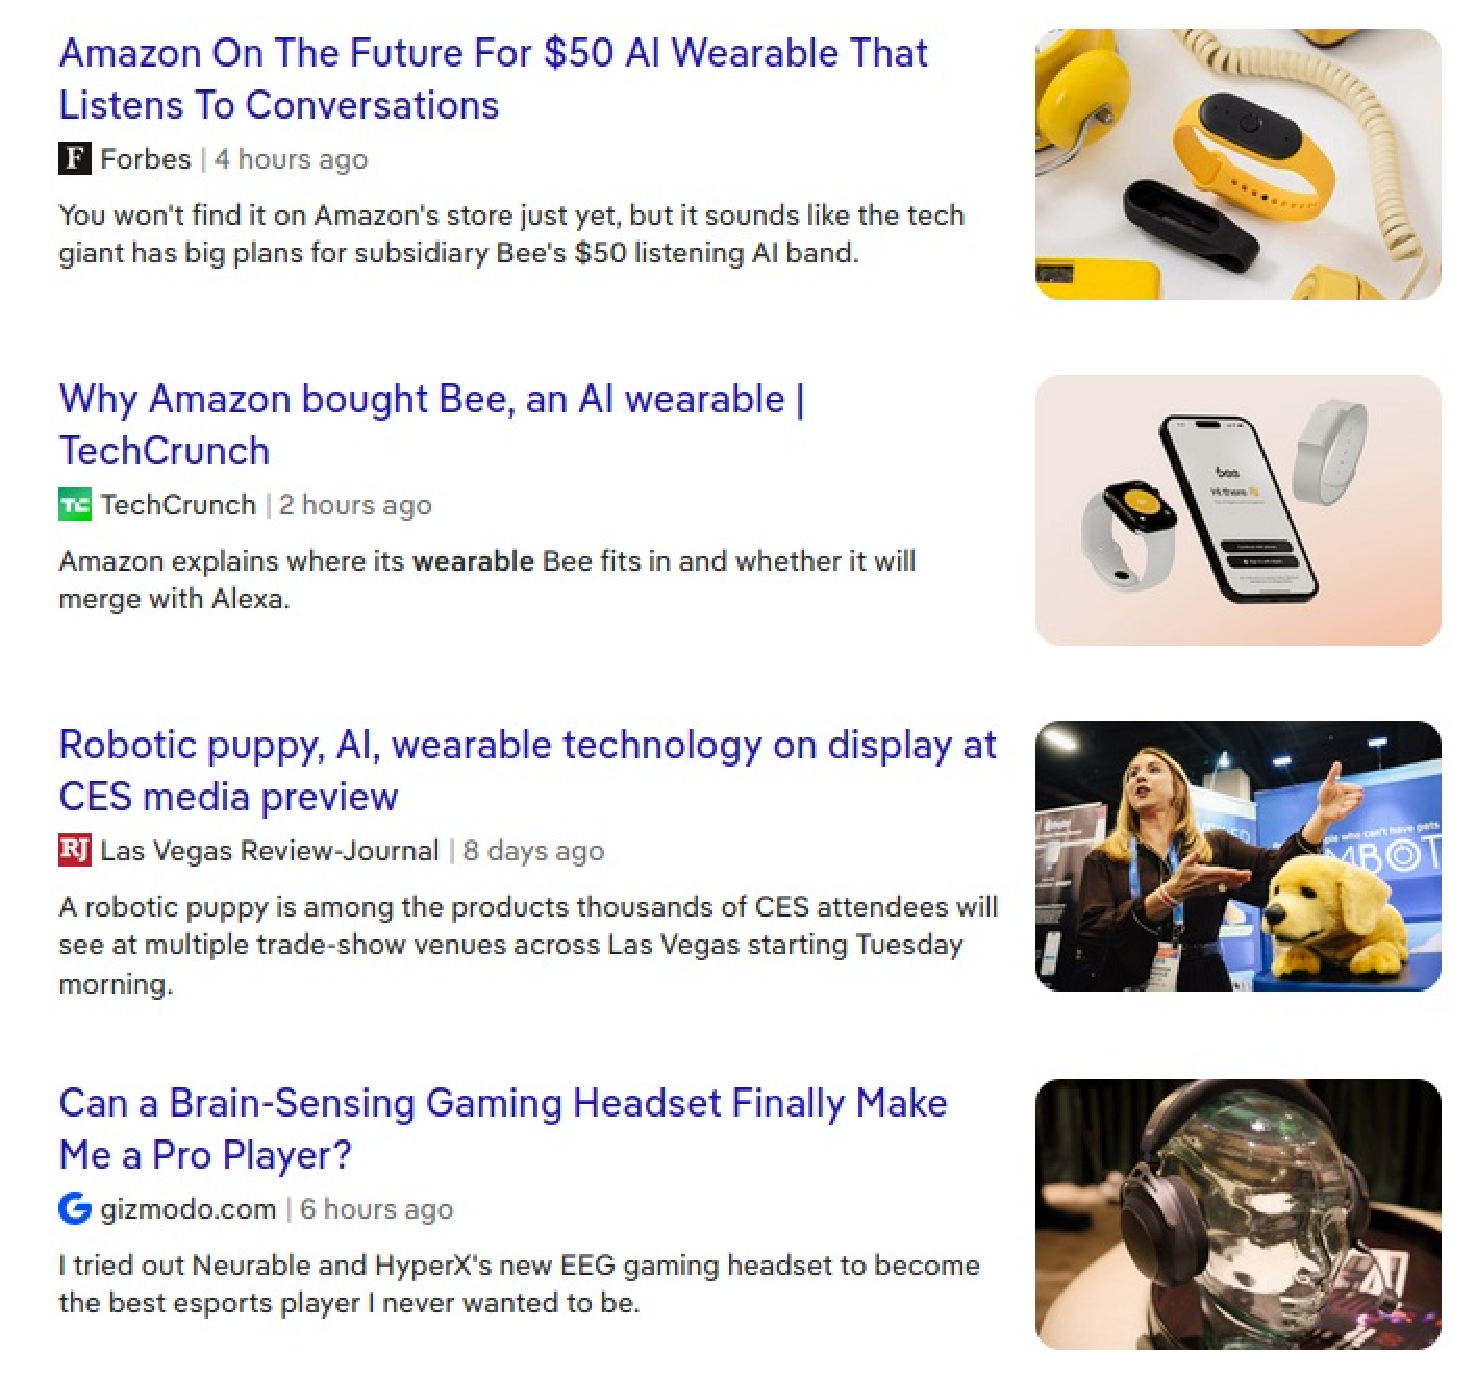
\includegraphics[width=0.45\textwidth]{figures/news1}
			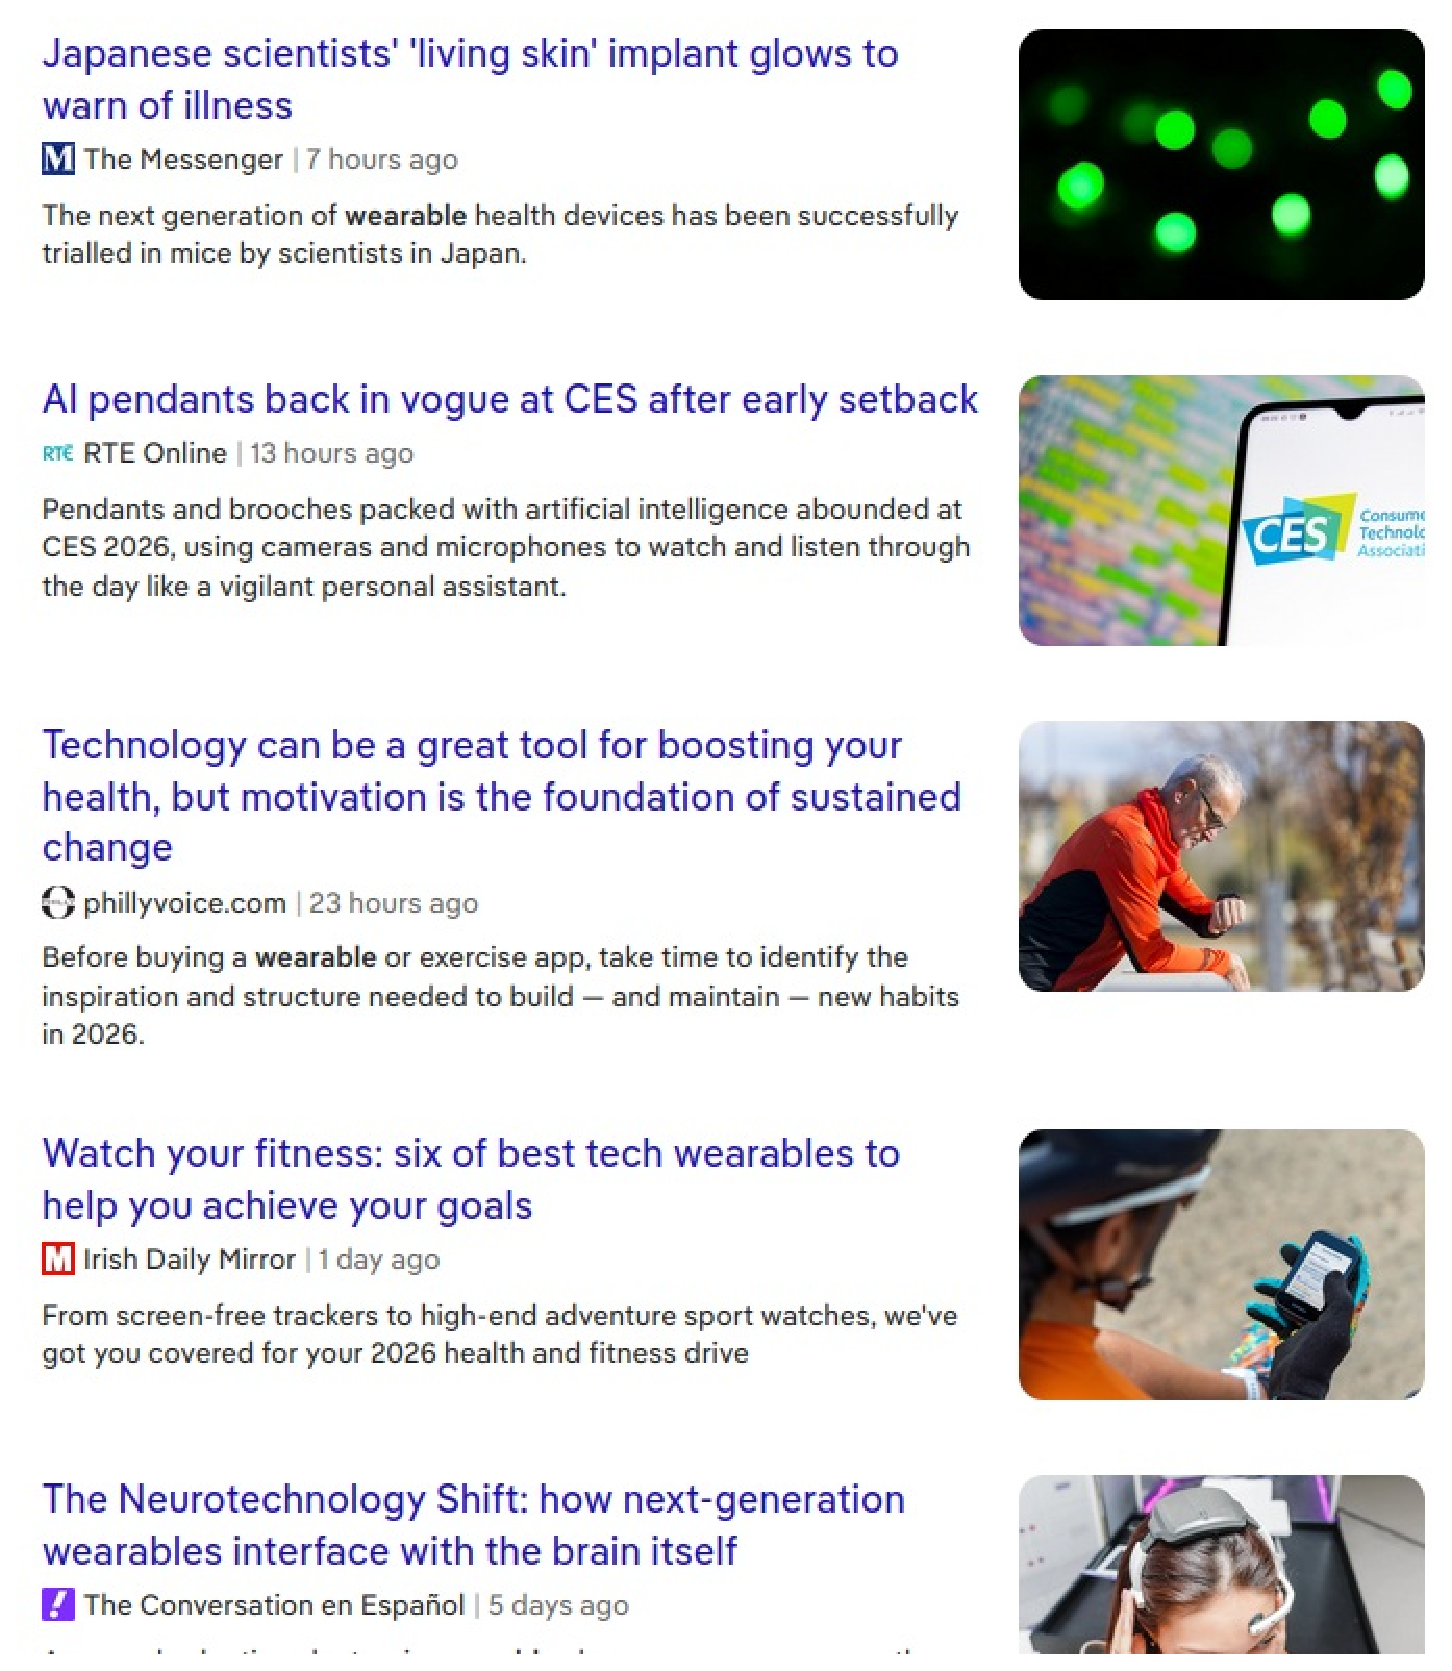
\includegraphics[width=0.45\textwidth]{figures/news2}
		\end{figure}
	\end{frame}
	
% 	\subsection{Some Examples}
% 	\begin{frame}
% 	\frametitle{Parkinson's Disease}
% 	\setbeamercovered{transparent=20}
% 	\begin{columns}[c]
% 		\column{2.5in}
% 		    \begin{itemize}
% 			 {\item Progressive degeneration of CNS}
% 			 {\item Disrupts proprioception}
% 			 {\item Effects gait/ambulation}
% 			      \begin{itemize}
% 				   {\item Freeze of Gait (FOG)}
% 			      \end{itemize}
% 			 {\item External cues supplement proprioception}
% 			      \begin{itemize}
% 				   {\item visual}
% 				   {\item auditory}
% 				   {\item \bf{vibratory}}
% 			      \end{itemize}
% 		    \end{itemize}
% 		\column{1.5in}
% 			\centering
% 			\begin{figure}
% 			      \centering
% 			      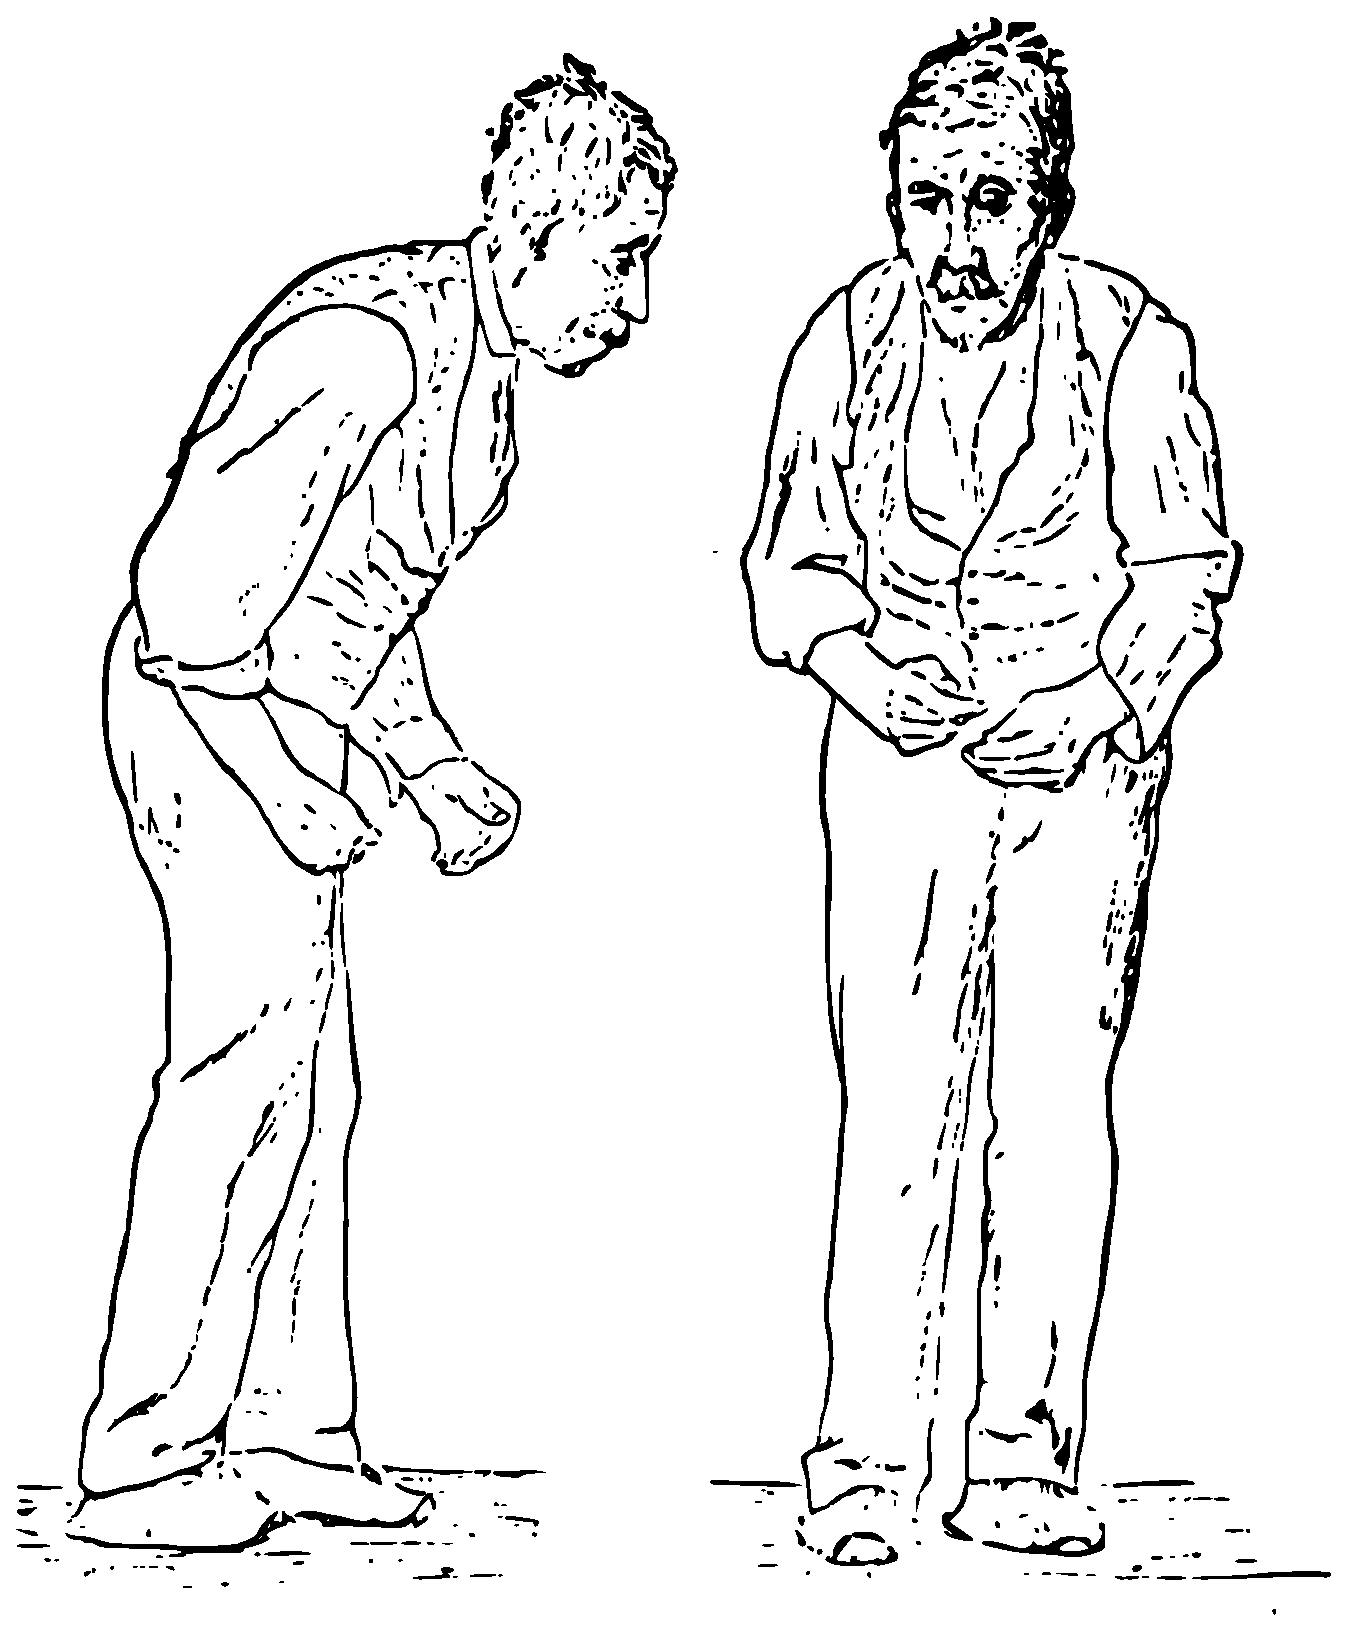
\includegraphics[width=1.25in]{figures/pd_sketch}
% % 			      \caption{Parkinson's disease as illustrated in \em A~Manual~of~Diseases of~the~Nervous~System\em.} % \footnote{http://commons.wikimedia.org/wiki/File:Sir\_William\_Richard\_Gowers\_Parkinson\_Disease\_sketch\_1886.svg}
% 			\end{figure}
% 	\end{columns}
% 	\end{frame}
%
% 	\begin{frame}
% 	\frametitle{Behavioral Health and Nutrition}
% 	Needs content
% 	\end{frame}
%
% 	\begin{frame}
% 	\frametitle{Brain Controlled Interfaces}
% 	Needs content
% 	\end{frame}
	
\section{Course Overview}
	\subsection{Course Objectives}
	\begin{frame}
	\frametitle{Undergraduate Course Objectives}
	\subsubsection{Undergraduate}
	Students who complete the undergraduate section of this course in good standing should be able to demonstrate the following advanced competencies:
\begin{enumerate}
	\item Select, assess, and apply techniques appropriate to the application of wearable technologies for healthcare and wellness applications;
	\item Synthesize, apply, and evaluate offline data analysis and machine learning techniques on large-scale data sets collected by wearable technologies;
	\item Identify, interpret, and critically explain the significance of open research areas in wearable technologies and their applications in health-driven research;
	\item Evaluate the applicability of wearable technologies in the commodity market.
\end{enumerate}

	\end{frame}

	\begin{frame}
	\frametitle{Graduate Course Objectives}
	\subsubsection{Graduate}
	Students who complete the graduate section of this course in good standing should be able to demonstrate the following advanced competencies:
\begin{enumerate}
	\item Select, assess, and apply techniques appropriate to the design and implementation of wearable technologies for healthcare and wellness applications, including specialized communication protocols and data structures and storage techniques;
	\item Synthesize, apply, and evaluate online and offline data analysis and machine learning techniques on large-scale data sets collected by wearable technologies;
	\item Identify, interpret, and critically explain the significance of open research areas in wearable technologies and their applications in health-driven research;
	\item Evaluate the applicability of wearable technologies in the commodity and research.
\end{enumerate}

	\end{frame}
	
	\subsection{Instructor}
	\begin{frame}
	\frametitle{Who am I?}
	\begin{wrapfigure}{L}{1.1in} % https://en.wikibooks.org/wiki/LaTeX/Floats,_Figures_and_Captions#Wrapping_text_around_figures
		\vspace{-.25in}
		\begin{center}
			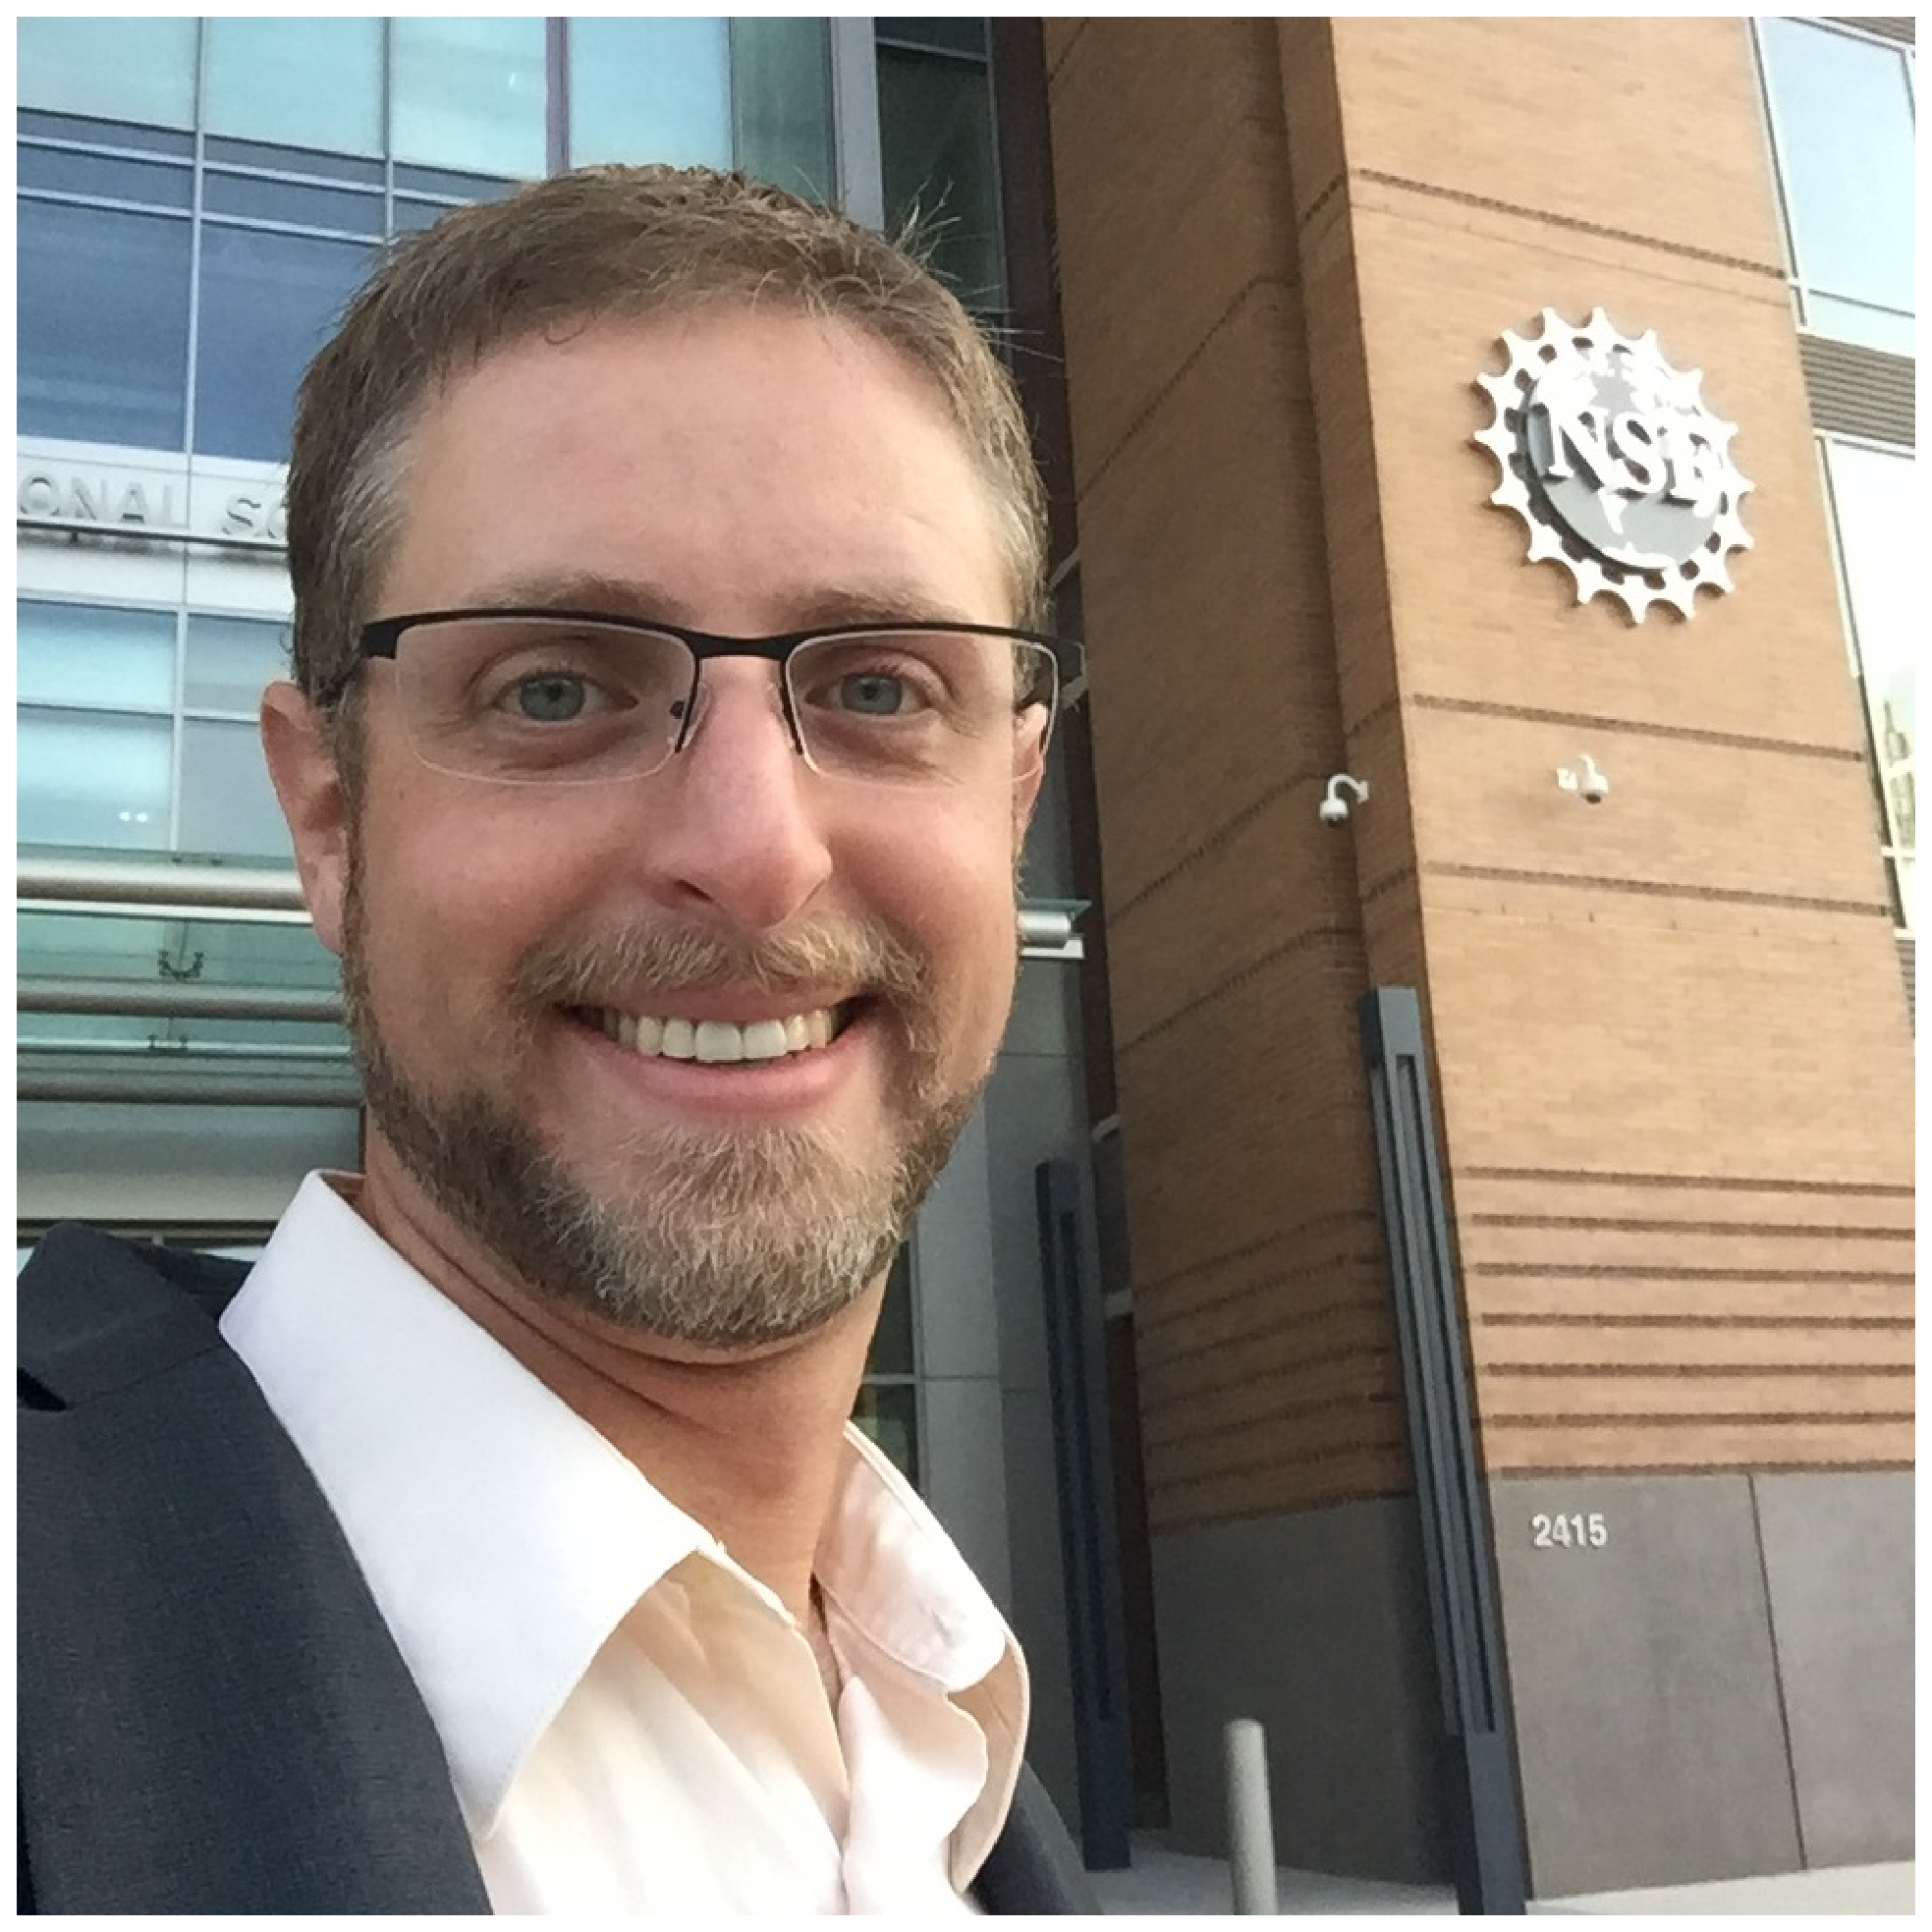
\includegraphics[width=1in, height=1.5in]{../syllabus/kyle}
		\end{center}
	\end{wrapfigure}
	Kyle N. Winfree, PhD

	Associate Professor

	Faculty of Informatics, Computer Science, and Electrical Engineering in the School of Informatics, Computing, and Cyber Systems

	Joined NAU in Fall of 2015

	AD of Undergrad Programs 2019-2022

	AD of Grad Programs 2022-2025
	\end{frame}
	
	\begin{frame}
	\frametitle{Formal Education and Training}
	\begin{itemize}
		\item NIH mHealth Training Institute Fellow
		\item Post-doc at Univ. of Delaware, PD intervention and assessment (SEnsole)
		\item Ph.D. at Univ. of Delaware in Biomechanics and Movement Science\\1.5 years focused on stroke rehabilitation robotics (ALEX)\\2.5 years dissertation on Parkinson’s disease rehabilitation (PDShoe)
		\item M.S.E. at Univ. of Pennsylvania in Robotics, thesis on haptics (iTorqU)
		\item US Geological Survey Astrogeology Branch, studied polar ice on Mars
		\item B.S. at \textbf{Northern Arizona University} in Physics
	\end{itemize}
	\end{frame}
	
	\begin{frame}
	\frametitle{PhD / Post Doc Topic: PDShoe / Sensole}
	\begin{figure}
		\includegraphics[width=0.3\textwidth]{figures/shoe}
		\includegraphics[width=0.3\textwidth]{figures/sensole}
		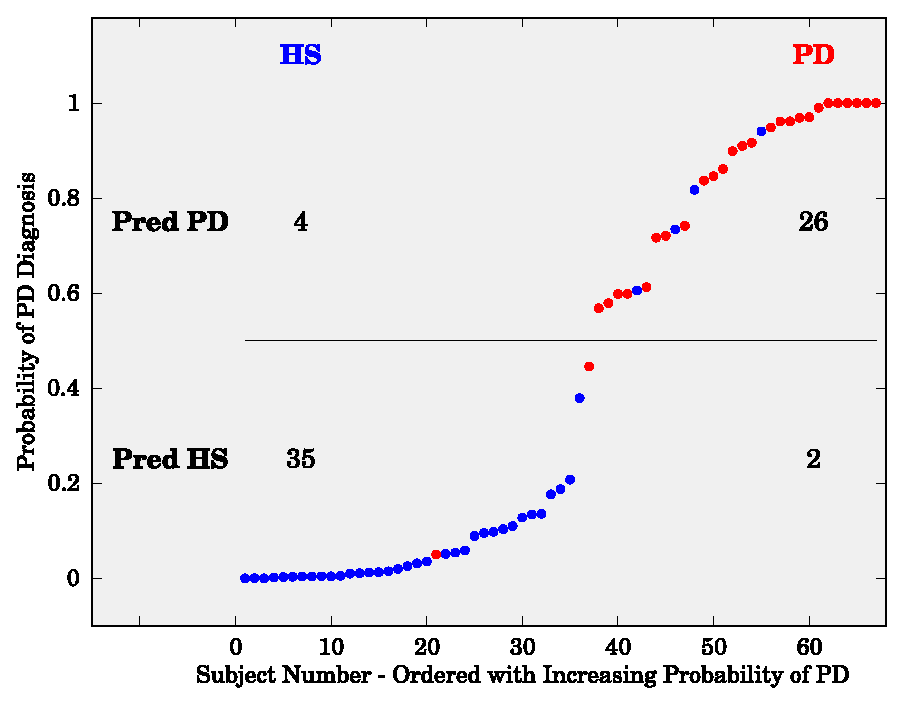
\includegraphics[width=0.3\textwidth]{figures/spss_results_ordered}
		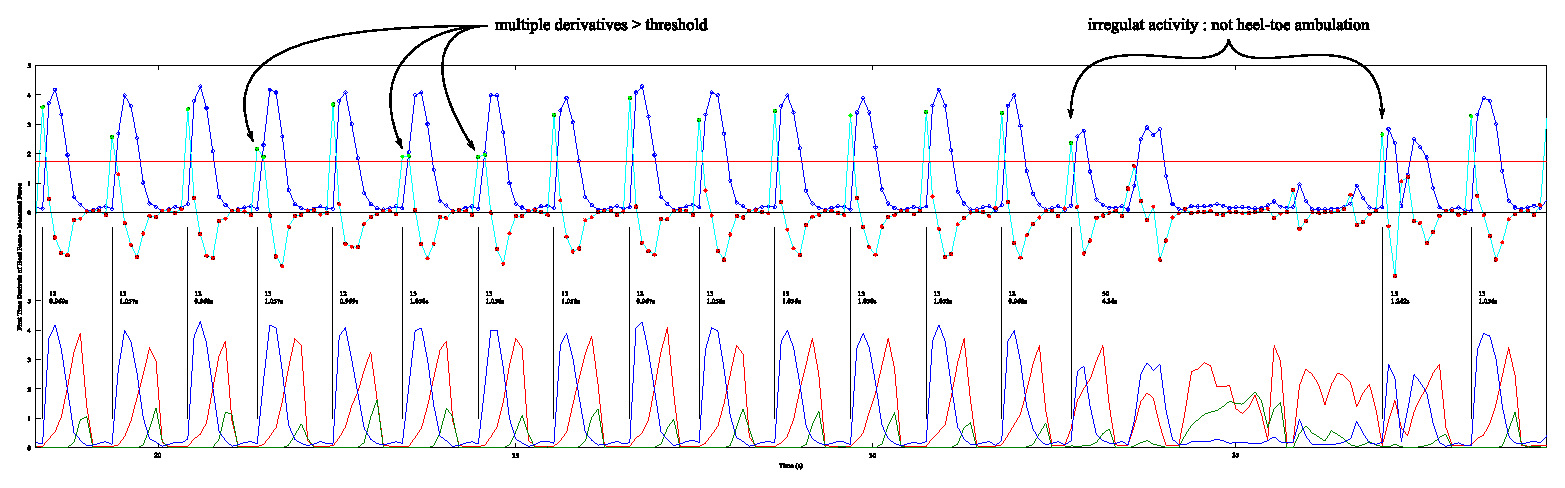
\includegraphics[width=0.90\textwidth]{figures/PD008_s1_test_strides_edit}
	\end{figure}
	\end{frame}
	
	\begin{frame}
	\frametitle{MS Thesis : iTorqU}
	\begin{figure}
		\includegraphics[width=0.23\textwidth]{figures/iTorqU1}
		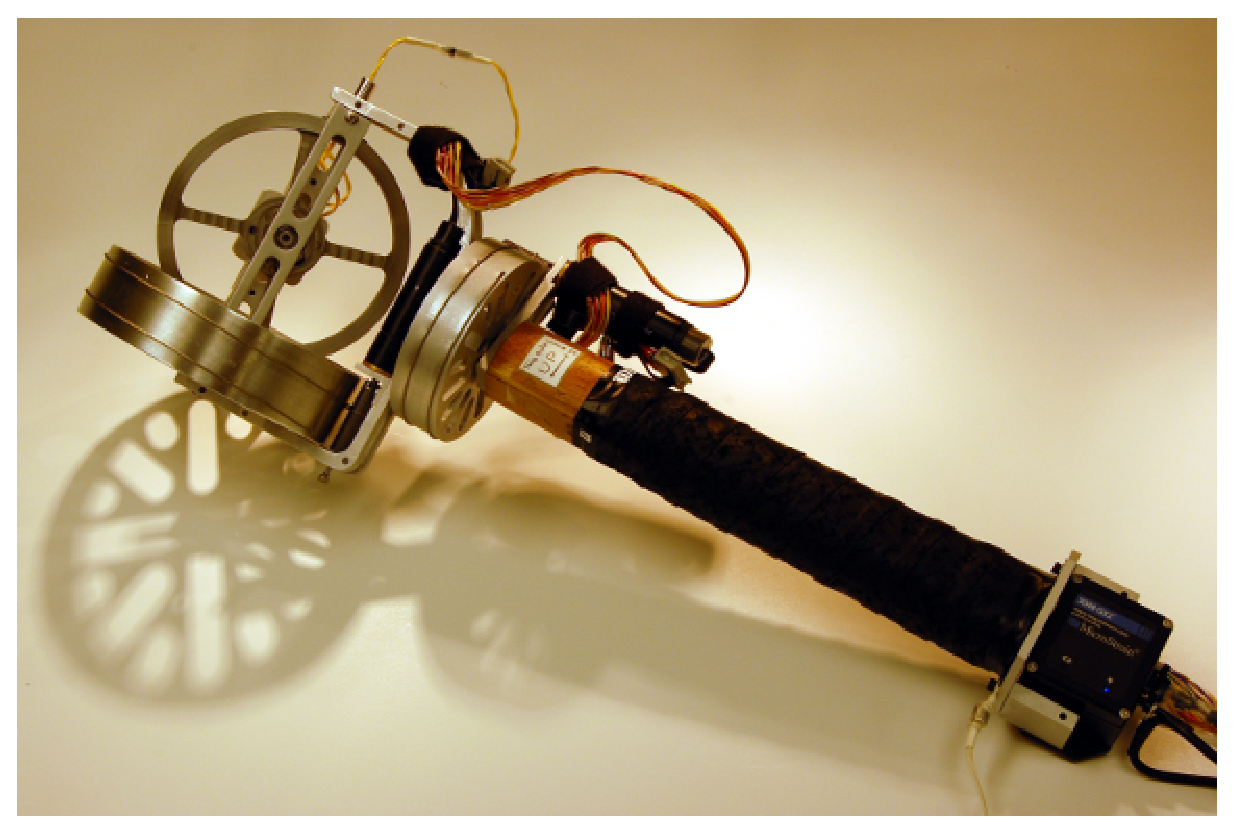
\includegraphics[width=0.73\textwidth]{figures/iTorqU2}
	\end{figure}
	\end{frame}
	
	\begin{frame}
	\frametitle{Research interests}
	\footnotesize
	\begin{itemize}
		\item Impact of Faculty Behaviors on Student-Faculty Rapport: A Multi-Institutional Study (2025)
		\item Optimizing Feature Extraction Methods Using Class Similarity Ratio for EMG-Based Hand Gesture Classification (2025, PhD Student)
		\item Ready, Set, Move! Tracking Children's Modified Ride-On Car Use With a Custom Data Logger (2023)
		\item Impact of Different Exercise Modalities on the Human Gut Microbiome (2021)
		\item Optimizing Student-Faculty Rapport for the Engineering Classrooms: Dimensioning the Behaviors that Matter (2020)
		\item The Development of an IoT Instrumented Bike: for Assessment of Road and Bike Trail Conditions (2018, PhD Student)
		\item Modeling Clinically Validated Physical Activity Assessments Using Commodity Hardware (2017)
		\item A novel method of assessing dietary behavior using a wrist-worn accelerometer (2017)
	\end{itemize}
	\normalsize
	\end{frame}
	
	\begin{frame}
	\frametitle{How do you contact me?}

	\textbf{Email:} \href{mailto:kyle.winfree@nau.edu}{kyle.winfree@nau.edu}

	\textbf{Canvas:} Better than email, send me a message on Canvas.  That will pop up on my phone.  I do NOT have email on my phone.
	
	\textbf{Office:} SICCS Room 204

	\textbf{In-Person:} Come see me in my office, stop me in the hallway, chat with me on a campus bus, etc.  I prefer in-person discussions for anything more than a 2 minute question / response.
	
	\textbf{Cell Phone:} 928.853.0114 \em{(please use this sparingly)}
	\end{frame}
	
\section{The Syllabus}
	\subsection{Canvas and Git}
	\begin{frame}
	\frametitle{Canvas and Git}
	\begin{itemize}
		\item Due dates for assignments will be on \href{https://canvas.nau.edu}{Canvas}
		\item Submission of assignments will be ``linked'' on Canvas (UG: Google Drive or GitHub, G: GitHub)
		\item Materials for class will be on \href{https://github.com/kylewinfree/inf632-spring2026}{GitHub/kylewinfree/inf632-spring2026}
		\begin{itemize}
			\item Look for an invite to join from me!
			\item Source for all course materials will also be in Canvas.  Graduate Students: I expect that you will typeset your assignment submissions; use this source to help you with \LaTeX.
		\end{itemize}
	\end{itemize}
	\end{frame}
	
	\subsection{Course Materials}
	\begin{frame}
	\frametitle{Course Materials}
	\begin{itemize}
		\item No text book will be required.
		\item You will need to purchase the materials to create a wearable device. This material list will be provided; expect costs to be approximately that of a textbook.
		\item Students in the undergraduate section have the option of completing the research project with off-the-shelf devices and may not need to purchase materials.
	\end{itemize}

	See the syllabus for recommended readings, including those that are available for free online.
	\end{frame}
	
	\subsection{Grading}
	\begin{frame}
	\frametitle{Grading}
	Graduate and Undergraduate students will be assessed with different rubrics (expectations).  The weight of each assignment is also different between these groups, owing to these different expectations.
	\tiny
	\begin{table}
    \begin{center}
    \caption{Assessments and related fractional percentage of final grade.\label{tab:percentage}}
        \begin{tabular}{lcc}
            \textbf{Assessment}									& \textbf{Undergraduate} & \textbf{Graduate} \\
            \toprule
            Attendance and in-class participation 				& 10\%			& 10\%\\
            \midrule[0.01em]
            Homework Assignments (3) 							& 45\% 			& 30\% \\
            \midrule[0.01em]
            Research Project: Literature Review 				& 5\% 			& 10\% \\
            Research Project: Questions and Hypotheses 			& 10\% 			& 10\% \\
            Research Project: Device Design and Implementation 	& 5\% 			& 10\% \\
            Research Project: Methods Plan 						& 5\% 			& 5\% \\
            Research Project: Analysis 							& 5\% 			& 10\% \\
            Research Project: Discussion of Findings 			& 10\% 			& 10\% \\
            Research Project: In-Class Presentation 			& 5\% 			& 5\% \\
            \bottomrule
            Total												& 100\%			& 100\%
        \end{tabular}
    \end{center}
\end{table}

	\normalsize
	\end{frame}
	
	\subsection{Participation Matters!}
	\begin{frame}
	\frametitle{Participation Matters!}
	I assume you are hear with the intention to learn something.

	With that assumption, then let's consider the following from J. E. Stice, ``Using Kolb's Learning Cycle to Improve Student Learning,'' Engineering Education, pp. 291-296, February 1987.
	\scriptsize
	\begin{table}
		\begin{center}
			\begin{tabular}{lcc}
				\textbf{Retention}	& \textbf{What one ...}	& \textbf{Class Activity} \\
				\toprule
				10\%				& reads			& Readings\\
				26\%				& hears			& Lectures\\
				30\%				& sees				& Figures, Drawings, Slides\\
				50\%				& sees and hears	& Lectures with Visuals\\
				70\%				& says				& Asking questions, Discussing papers\\
				90\%				& says while doing	& Hands-on activities, Project demos\\
				\bottomrule
			\end{tabular}
		\end{center}
	\end{table}
	\normalsize
	So come to class, for every lecture, every lab, and every project ``office'' hours!
	\end{frame}
	
	\subsection{Office Hours}
	\begin{frame}
	\frametitle{Office Hours}
	Class is on Tuesday and Thursday

	It seems like Thursday afternoon, Friday morning, or Monday might be good office hours candidates.

	So let's survey you!

	\begin{table}
		\begin{center}
			\begin{tabular}{l | c}
				Thursday 12:45-2:00 & ? \\
				Thursday 2:30-3:45 & ? \\
				Friday 9:00-10:15 & ? \\
				Friday 10:00-11:15 & ? \\
				Monday 1:00-2:15 & ? \\
				Monday 2:00-3:15 & ? \\
			\end{tabular}
		\end{center}
	\end{table}
	\end{frame}
	
	\subsection{Schedule}
	\begin{frame}
	\frametitle{Schedule}
	See the syllabus for a complete and readable version =)
	\tiny
	\begin{table}[ht!]
\begin{center}
\caption{Tentative Course Schedule.\label{tab:schedule}}
\begin{tabular}{c p{4in}}
\textbf{Week of} & \textbf{Content} \\
\toprule

% this tex file includes the defs for due dates, making it possible to update this file each semester and have all the dates automatically reflect in all docs.

% pgfmath might be a better approach.
% or a python script that takes a few inputs and then generates this file.

% week 1
\def \wkOneMo{January 12} % course intro, reading
\def \wkOneTu{January 13}
\def \wkOneTh{January 15} % HW1 assigned

% week 2
\def \wkTwoMo{January 19} % this is generally MLK day
%                           dims of func, hapitcs
\def \wkTwoTu{January 20}
\def \wkTwoTh{January 22}

% week 3
\def \wkThreeMo{January 26} % health trends, analysis, compare testing
\def \wkThreeTu{January 27}
\def \wkThreeTh{January 29} % HW1 due, HW2 assigned

% week 4
\def \wkFourMo{February 2} % intro of RP, res methods for studies
\def \wkFourTu{February 3}
\def \wkFourTh{February 5}

% week 5
\def \wkFiveMo{February 9} % Lit rev, hypothesis, no class Thurs (2026)
\def \wkFiveTu{February 10} % RP-lit review assigned
\def \wkFiveTh{February 12}

% week 6
\def \wkSixMo{February 16} % Statistical learning, regression, fitting, NNs
\def \wkSixTu{February 17}
\def \wkSixTh{February 19} % HW2 due, HW3 assigned

% week 7
\def \wkSevenMo{February 23} % Stat Learn SVM, trees, k-means, knn
\def \wkSevenTu{February 24} % RP-lit review due, RP-Q&H assigned
\def \wkSevenTh{February 26}

% week 8
\def \wkEightMo{March 2} % device design, sensing
\def \wkEightTu{March 3} % RP-Q&H due, RP-design assigned
\def \wkEightTh{March 5}

% spring break
\def \springBreakMo{March 9} % NADA
\def \springBreakFr{March 13} % RIEN
%\def \springBreakTh{March 12}

% week 9
\def \wkNineMo{March 16} % soldering lab, arduino pt 1
\def \wkNineTu{March 17}
\def \wkNineTh{March 19} % HW3 due

% week 10
\def \wkTenMo{March 23} % arduino pt 2, raspberry pi
\def \wkTenTu{March 24} % RP-design due, RP-methods assigned
\def \wkTenTh{March 26}

% week 11
\def \wkElevenMo{March 30} % project time
\def \wkElevenTu{March 31} % RP-methods due, RP-analysis assigned
\def \wkElevenTh{April 2}

% week 12
\def \wkTwelveMo{April 6} % project time
\def \wkTwelveTu{April 7}
\def \wkTwelveTh{April 9}

% week 13
\def \wkThirteenMo{April 13} % interp results, communicating findings
\def \wkThirteenTu{April 14} % RP-analysis due, RP-discuss assigned
\def \wkThirteenTh{April 16}

% week 14
\def \wkFourteenMo{April 20} % writing lab
\def \wkFourteenTu{April 21} % RP-discuss due, RP-pres assigned
\def \wkFourteenTh{April 23}

% week 15
\def \wkFifteenMo{April 27} % project time
\def \wkFifteenTu{April 28} %RP-pres due
\def \wkFifteenTh{April 30}

% week 16 - Finals Week
\def \finalsWeekMo{May 4}
\def \finalsDay{May 7}
\def \finalsTime{10:00am to 12:00pm}
% \def \wk16Th{January 15}


% January %%%%%%%%%%%%%%%%%%%%%%%%%%%%%%%%%%%%%%%%%%%%%%% Week 1
	January 12 & \begin{minipage}{4in}
	Course expectations, setup (GitHub or Google Drive), and peer introductions (come prepared to introduce yourself with something you learned this past semester or summer).\\
	Start your assigned reading --- this should become habit!
	\end{minipage} \\
	\midrule[0.01em]
%%%%%%%%%%%%%%%%%%%%%%% Week 2
	January 19 & \begin{minipage}{4in}
	Dimensions of functionality\\
	Haptic interfaces\\
	\em{NAU is closed on Monday in observance of MLK Day}
	\end{minipage} \\
	\midrule[0.01em]
%%%%%%%%%%%%%%%%%%%%%%% Week 3
	January 26 & \begin{minipage}{4in}
	Health research and trends in wearable health monitoring\\
	Analysis, comparative testing
	\end{minipage} \\
	\midrule[0.01em]
% February %%%%%%%%%%%%%%%%%%%%%%%%%%%%%%%%%%%%%%%%%%%%%%% Week 4
	February 2 & \begin{minipage}{4in}
	Introduction of the {\bf Research Project}\\
	Research methods for studies\\
	\end{minipage} \\
	\midrule[0.01em]
%%%%%%%%%%%%%%%%%%%%%%% Week 5
	February 9 & \begin{minipage}{4in}
	Literature review, finding the gap in knowledge, forming a hypothesis\\
	No class on Thursday!
	\end{minipage} \\
	\midrule[0.01em]
%%%%%%%%%%%%%%%%%%%%%%% Week 6
	February 16 & \begin{minipage}{4in}
	Statistical learning methods (applied) --- regression, logistic regression, over fitting, neural nets
	\end{minipage} \\
	\midrule[0.01em]
%%%%%%%%%%%%%%%%%%%%%%% Week 7
	February 23 & \begin{minipage}{4in}
	Statistical learning methods (applied) --- support vector machines, decision trees, k-means, k-nearest neighbors
	\end{minipage} \\
	\midrule[0.01em]
%%%%%%%%%%%%%%%%%%%%%%% Week 8
	March 2 & \begin{minipage}{4in}
	Device design\\
	Sensing\\
	\end{minipage} \\
	\midrule[0.01em]
% March %%%%%%%%%%%%%%%%%%%%%%%%%%%%%%%%%%%%%%%%%%%%%%%
	March 9 & \begin{minipage}{4in}
	Spring Break! No class.
	\end{minipage} \\
	\midrule[0.01em]
%%%%%%%%%%%%%%%%%%%%%%% Week 9
	March 16 & \begin{minipage}{4in}
	Soldering lab\\
	Arduino Part 1\\
	Device design review (everyone shares)
	\end{minipage} \\
	\midrule[0.01em]
%%%%%%%%%%%%%%%%%%%%%%% Week 10
	March 23 & \begin{minipage}{4in}
	Arduino Part 2\\
	Raspberry Pi
	\end{minipage} \\
	\midrule[0.01em]
%%%%%%%%%%%%%%%%%%%%%%% Week 11
	March 30 & \begin{minipage}{4in}
	Project time
	\end{minipage} \\
	\midrule[0.01em]
% April %%%%%%%%%%%%%%%%%%%%%%%%%%%%%%%%%%%%%%%%%%%%%%% Week 12
	April 6 & \begin{minipage}{4in}
	Project time
	\end{minipage} \\
	\midrule[0.01em]
%%%%%%%%%%%%%%%%%%%%%%% Week 13
	April 13 & \begin{minipage}{4in}
	Interpreting your results\\
	Communicating your analyses and findings
	\end{minipage} \\
	\midrule[0.01em]
%%%%%%%%%%%%%%%%%%%%%%% Week 14
	April 20 & \begin{minipage}{4in}
	Writing lab --- come prepared to work on writing up the {\bf Discussion and Findings} with your group
	\end{minipage} \\
	\midrule[0.01em]
%%%%%%%%%%%%%%%%%%%%%%% Week 15
	April 27 & \begin{minipage}{4in}
	Project time
	\end{minipage} \\
	\midrule[0.01em]
% May %%%%%%%%%%%%%%%%%%%%%%%%%%%%%%%%%%%%%%%%%%%%%%% Finals Week
	May 4 & \begin{minipage}{4in}
	Finals week, no class on Tuesday\\
	Project presentations on Thursday from 10:00am to 12:00pm
	\end{minipage} \\
	\midrule[0.01em]
\end{tabular}
\end{center}
\end{table}

	\normalsize
	\end{frame}
	
\section{Class Composition and Goals}
	\subsection{Who are you?}
	\begin{frame}
	\frametitle{Who are you?}
	\begin{enumerate}
		\item Your name
		\item Are you an Undergrad, Grad MS, Grad PhD, or... ?
		\item Your Major
		\item What might come after said degree?
		\item Are you enrolled for credit or auditing?
		\item Why are you here?
		\item What are your research interests?
		\item What is something you learned this past semester or summer?
	\end{enumerate}
	\end{frame}

\end{document}
